\documentclass[12pt]{article}

\usepackage{graphicx}
\usepackage{amsmath}
\usepackage{pdfpages}


\begin{document}
\begin{titlepage}
\centering
\vfill
\textbf{\Huge{Assignment Report }}\\
\vskip 1cm
\textbf{\Huge{Telecommunication Software Lab  \linebreak \\ELP 718}}\\
\vskip 1cm
\textbf{\Large{\underline{\emph{Name: Anupam Kumar Jha}}}}\\
\vskip 0.5cm
\textbf{\Large{\underline{\emph{Entry number: 2016JTM2087}}}}
\vskip 0.5cm
\textbf{\Large{\underline{\emph{Assignment no. 12}}}}
\vskip 1cm
\Large{\textbf{\emph{Submission Date: November 3, 2016}}}
\vskip 1.5cm

\includegraphics[scale=0.3]{logo.png}
\vskip 0.5cm
\textbf{\emph{Indian Institute of Technology}}\\
\textbf{\emph{Delhi}}\\
     
November 3, 2016
\vfill 
\end{titlepage} 


\begin{center}
\tableofcontents
\end{center}

\newpage
\listoffigures
\newpage

\section{Introduction}


  Lex is officially known as a "Lexical Analyser".

It's main job is to break up an input stream into more usable elements.
Or in, other words, to identify the "interesting bits" in a text file.

For example, if you are writing a compiler for the C programming language, the symbols $\{ \}$ , ( ) ; all have significance on their own. The letter a usually appears as part of a keyword or variable name, and is not interesting on it's own. Instead, we are interested in the whole word. Spaces and newlines are completely uninteresting, and we want to ignore them completely, unless they appear within quotes "like this".

All of these things are handled by the Lexical Analyser. 


  Yacc is officially known as a "parser".It's job is to analyse the structure of the input stream, and operate of the "big picture".In the course of it's normal work, the parser also verifies that the input is syntactically sound.Consider again the example of a C-compiler. In the C-language, a word can be a function name or a variable, depending on whether it is followed by a ( or a $=$ There should be exactly one \} for each \{ in the program.

YACC stands for "Yet Another Compiler Compiler". This is because this kind of analysis of text files is normally associated with writing compilers.










\newpage
\section{Problem Statements}

\subsection{Problem Statement 1}
We have to write a lex/yacc code to evaluate the consistency of given .pgn file, which record chess moves in given game. You have to find any wrong notations and its location in metadata or using move number. The PGN file follows international notation rules. THE PGN file has metadat and record of pawn moves.

\subsection{Problem Statement 2}
We are given list of students in given format with their marks in respective subjects. We have to calculate their SGPA and write that down after every student. Input file has entry number, name of student, followed by marks in respective subjects.


\newpage

\section{Assumptions}
\subsection{Assumptions for Problem Statement 1}
Assumptions for problem statement 1 are:
\begin{itemize}
\item Assumption no $1$ : The matadata of PGN file has only seven fields.
\item Assumption no $2$ : The chess moves are not to be validated. Only the syntax of the recorded chess moves is to be validated.
\end{itemize}

\subsection{Assumptions for Problem Statement 2}
Assumptions for problem statement 2 are:
\begin{itemize}
\item Assumption no $1$ : SGPA is calcualted using IIT Delhi rules. 
\item Assumption no $2$ : Dropped and Audit course are not taken into account while  calculating SGPA.
\end{itemize}
\newpage

\newpage

\section{Logic and Impletantaion}
\subsection{Implementation for Problem Statement 1}
\begin{itemize}
\item
Write regular expressions to check the metadata. There are seven fields and specific input formats to check.
\item
Write regular expression for chess moves. Consider only normal moves where no peice is killed.
\item
Consider case where some piece is killed. Write regex for that.
\item
Declare variables val and inval, mvno, nmeta, count. Initialize all to zero. 
\item
Increment mvno whenever regex for valid index is detected. Increment val whenever valid pattern is detected. IF mvno and val are not equal, error has occured. 
\item
Similarly, nmeta is incremented whenever valid meta data  is detected. At the end, if nmeta is less than 7, there is error in meta data.

\end{itemize}
\subsection{Implementation for Problem Statement 2}
\begin{itemize}
\item
Write regular expressions to check the input file format. 
\item
When the format is proper, copy the line to output file.
\item
Extract credits obtained and the weightage of each subject using appropriate field position. Do weighted sum and divide by no of subjects to get the SGPA.



\end{itemize}



\newpage



\section{Test Description and Results}
\subsection{Tests for Problem Statement 1}
The code runs properly as asked for:
\begin{itemize}
\item
When a standard file is given in input, no error is displayed. 
\item
Introduce an error at move no 20 by giving a specail symbol. The output will show invalid data at move 20.
\item
Similarly, introduce a format error at any other move no. Error is displayed for that perticular move no.
\item
If admin is logged in, Marks button displays students marks graph.

\end{itemize}

\subsection{Tests for Problem Statement 2}
The code runs properly as asked for:
\begin{itemize}
\item
Give entry no with invalid year. It displays error.
\item
Give a literal in place of number for grade. Error is displayed.
\item
Give 3 students' data with 2 or more subjects. SGPA is properly displayed.
\item
Use Dropped and audit courses. The output does not count them for calculating SGPA.

\end{itemize}




\newpage
\section{Screenshots}

Following are the screenshots for program output:

\begin{figure}[h]

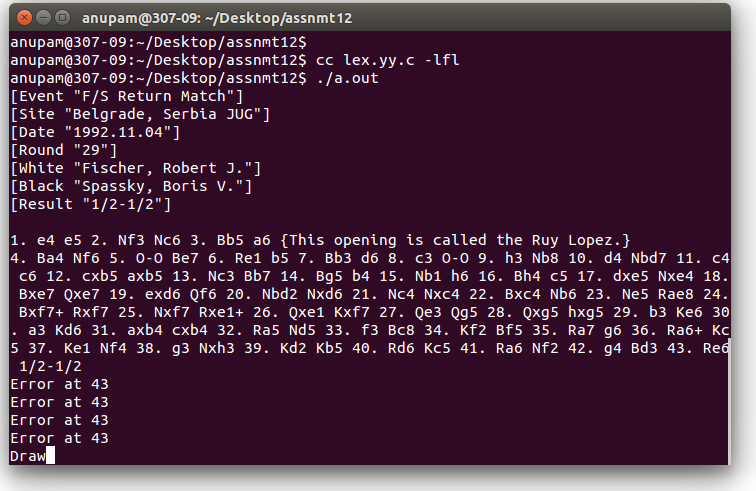
\includegraphics[scale=0.6]{ps1.png}
\caption{Screenshot1 for problem statement 1}
\end{figure}


\newpage

\begin{figure}[h]
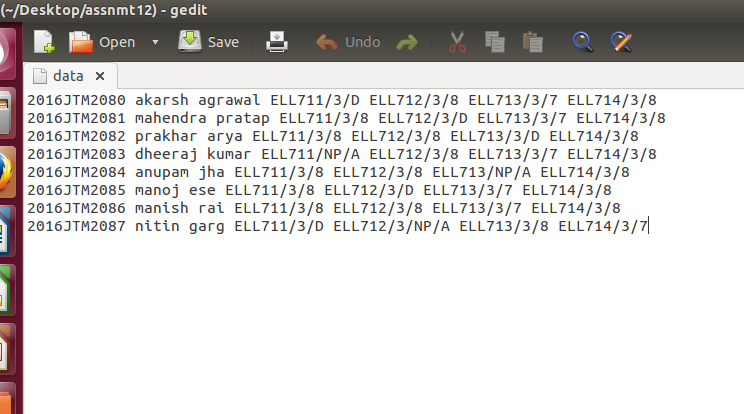
\includegraphics[scale=0.65]{ps21.png}
\caption{Screenshot2 for problem statement 2 (1st fig)}
\end{figure}

\newpage

\begin{figure}[h]
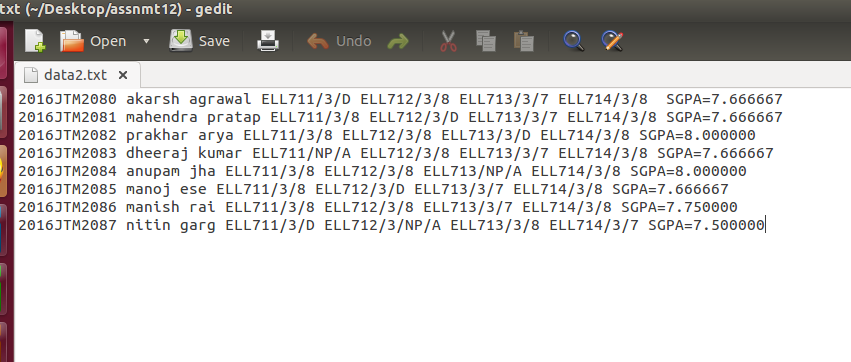
\includegraphics[scale=0.65]{ps22.png}
\caption{Screenshot2 for problem statement 2 (2nd fig)}
\end{figure}

\newpage

\begin{figure}[h]
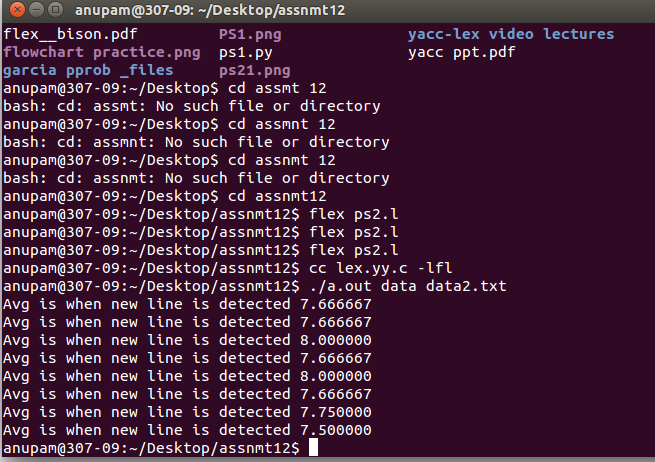
\includegraphics[scale=0.65]{ps23.png}
\caption{Screenshot2 for problem statement 2 (3rd fig)}
\end{figure}




\newpage

\section{References and citations}
\begin{thebibliography}{3} 

\bibitem{Online1}
Online reference for LEX and YACC. Available: http://dinosaur.compilertools.net/

\bibitem{Online2}
LEX and YACC tutorial. Availabe: http://epaperpress.com/lexandyacc/download/LexAndYaccTutorial.pdf


\bibitem{Online2}
Basic introduction to LEX and YACC. Available: https://luv.asn.au/overheads/lex\_ yacc/



 
\end{thebibliography}



\newpage
\section{\textbf{Epilogue}}
This assignment has taught us use of LEX and YACC for basic text processing.

\end{document}